\documentclass[12pt]{article}

%\usepackage[spanish]{babel}
\usepackage{amsmath,latexsym,amssymb}

\usepackage{graphicx}

\usepackage{geometry}
%\usepackage{showframe} %This line can be used to clearly show the new margins
%\newgeometry{vmargin={15mm}, hmargin={12mm,17mm}}   % set the margins
%\newgeometry{vmargin={20mm}, hmargin={20mm,20mm}}   % set the margins
\newgeometry{vmargin={20mm}, hmargin={20mm,20mm}}

\newcommand{\R}{\mathbb{R}}

\usepackage{subcaption}

%\newcommand{\aa}{\'{a}}
%\newcommand{\'i}{\'{\i}}
%\newcommand{\o}{\'{o}}

\begin{document}

\begin{center}

{\Large{\underline{\bf En memoria de Peter Higgs (1929 -- 2024)}}} \vspace*{2mm} \\

\end{center}

\noindent
Peter Higgs fue un f\'isico te\'orico brit\'anico, famoso por su
trabajo de 1964 donde propuso un mecanismo que puede generar masas
para part\'iculas elementales, conforme a la simetr\'{\i}a de norma.
Medio siglo despu\'es, dos experimentos del CERN confirmaron
que este mecanismo est\'a realizado en la naturaleza.
El 8 de abril nos lleg\'{o} la triste noticia del fallecimiento del
gran pionero de la f\'{\i}sica de part\'{\i}culas elementales.
Este art\'{\i}culo es dedicado a su memoria, al mecanismo
y la part\'icula que llevan su nombre.

\section{Datos biogr\'aficos y contexto hist\'orico}

Peter Higgs naci\'o en 1929 en Newcastle, Inglaterra, por lo qu\'e
pas\'{o} su juventud parcialmente durante la Segunda Guerra Mundial,
circunstancias que complicaron un poco su formaci\'on escolar.
Despu\'es de la guerra, estudi\'o en Londres, primero matem\'aticas,
luego f\'isica. En 1954, con s\'olo 25 a\~nos termin\'o su
doctorado en el {\it King's College.}

Luego trabaj\'{o} temporalmente en la Universidad de Edimburgo,
en el {\it University College} y en el {\it Imperial College,} ambos
en Londres.
En 1960 regres\'{o} a Edimburgo -- ciudad que le encant\'o y donde
hab\'ia llegado por primera vez en 1949, como estudiante viajando
con {\it auto-stop} -- para ocupar un puesto de catedr\'{a}tico y
quedarse ah\'{\i} toda su vida.

En 1964, a los 35 a\~{n}os, escribi\'o sus dos art\'{\i}culos famosos
(y otro sobre el mismo tema en 1966) \cite{Higgs} que llamaron la
atenci\'{o}n y condujeron a invitaciones para presentar seminarios en
Princeton y Harvard en 1966. Ten\'{\i}a que tratar con audiencias cr\'iticas,
Sidney Coleman coment\'{o} m\'{a}s tarde que en Harvard ``quer\'ian
romper en pedazos al idiota que pensaba que pod\'ia evadir el
Teorema de Goldstone'' \cite{boson}. Result\'{o} que su concepto sigu\'io
de pie, pero a\'un sin aplicaci\'{o}n fenomenol\'{o}gica
(sus art\'iculos trataron con un modelo de juguete). Adem\'{a}s
se enter\'{o} por Yoichiro Nambu (el \'arbitro de uno de sus
art\'iculos) de un trabajo parecido \cite{EB}, publicado
15 d\'ias antes del primer art\'iculo de Higgs sobre el tema.
Los autores eran Fran\c{c}ois Englert y Robert Brout quienes
trabajaron en Bruselas, B\'elgica. Dos meses despu\'{e}s apareci\'{o}
otro art\'{\i}culo relacionado, escrito en Londres por
Gerald Guralnik, Carl Hagen y Tom Kibble \cite{GHK}, pero ellos
conocieron y citaron los trabajos anteriores de Englert, Brout y Higgs.



El mecanismo que estos tres art\'{\i}culos propusieron no era
totalmente nuevo: hab\'ia sido establecido en 1962/3 en el contexto de la
materia condensada por Philip Anderson \cite{Anderson}. \'El aplic\'o
conceptos de Julian Schwinger \cite{Schwinger} para la explicaci\'on
te\'orica de la masa de una part\'icula de norma a la teor\'ia de
superconductores. Englert, Brout y Higgs presentaron una
extensi\'on a modelos relativistas.

\begin{figure}[h]
	\centering
	\begin{subfigure}{0.3\textwidth}
	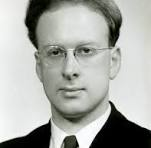
\includegraphics[scale=0.8]{images/higgs_joven.jpeg}
	\caption{}
	\end{subfigure}
	\begin{subfigure}{0.6\textwidth}
	\centering
	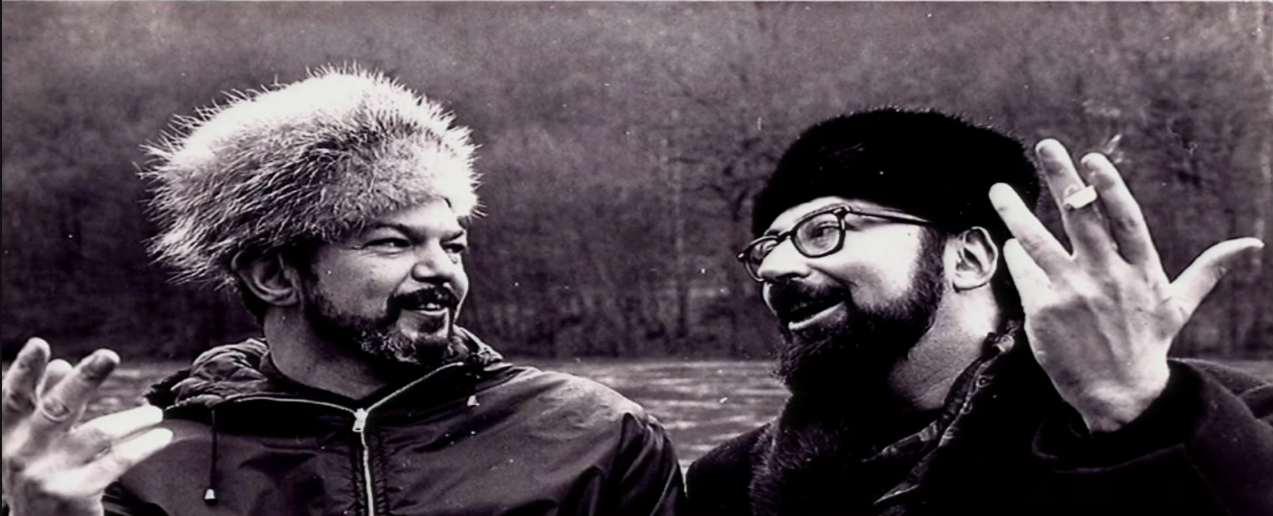
\includegraphics[scale=0.25]{images/brout_englert.png}
	\caption{}
	\end{subfigure}
	\caption{(a) Peter Higgs, quien public\'o dos art\'iculos breves sobre
        el ahora llamdo mecanismo de Higgs en 1964, y otro m\'as extenso
        en 1966. (b) Robert Brout
        (izquierda) y Fran\c{c}ois Englert (derecha). Brout invit\'o a
        Englert a trabajar en la Universidad de Cornell en 1959 por
        dos años como investigador asociado. Despu\'es
        Brout y Englert dejaron Cornell para trabajar en la
        Universidad de Bruselas, B\'elgica.}
	\end{figure}
\begin{figure}
\centering
\begin{subfigure}{0.31\textwidth}
	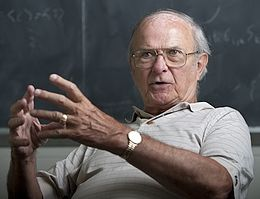
\includegraphics[scale=2]{images/hagen.jpg}
\end{subfigure}	
\begin{subfigure}{0.31\textwidth}
	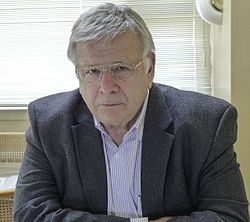
\includegraphics[scale=0.5]{images/guralnik.jpg}
\end{subfigure}	
\begin{subfigure}{0.31\textwidth}
	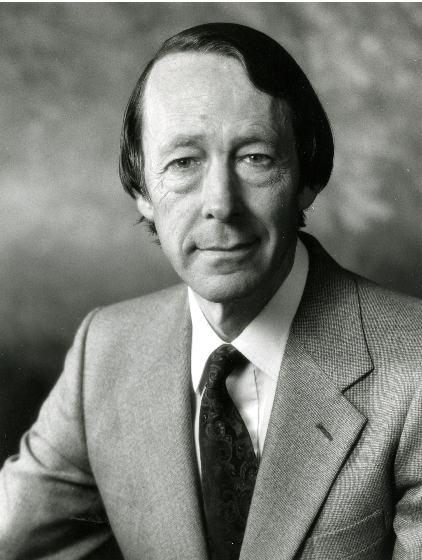
\includegraphics[scale=0.25]{images/kibble.png}
\end{subfigure}	

	\caption{Los otros descubridores del mecanismo de Higgs.
        De izquierda a derecha, Carl Hagen, Gerald Guralnik y Tom Kibble.} 
\end{figure}

\begin{figure}[h]
\centering
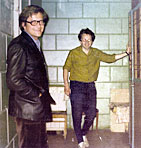
\includegraphics[scale=1]{images/polyakov_migdal.jpg}	
\caption{Cuando a\'un eran {\it teenagers}, Alexander
Migdal (izquierda) y Alexander Polyakov (derecha) descubrieron
independiente del occidente el principio del mecanismo de Higgs.}
\end{figure}


	\begin{figure}
			\begin{subfigure}{0.5\textwidth}
	\centering	
		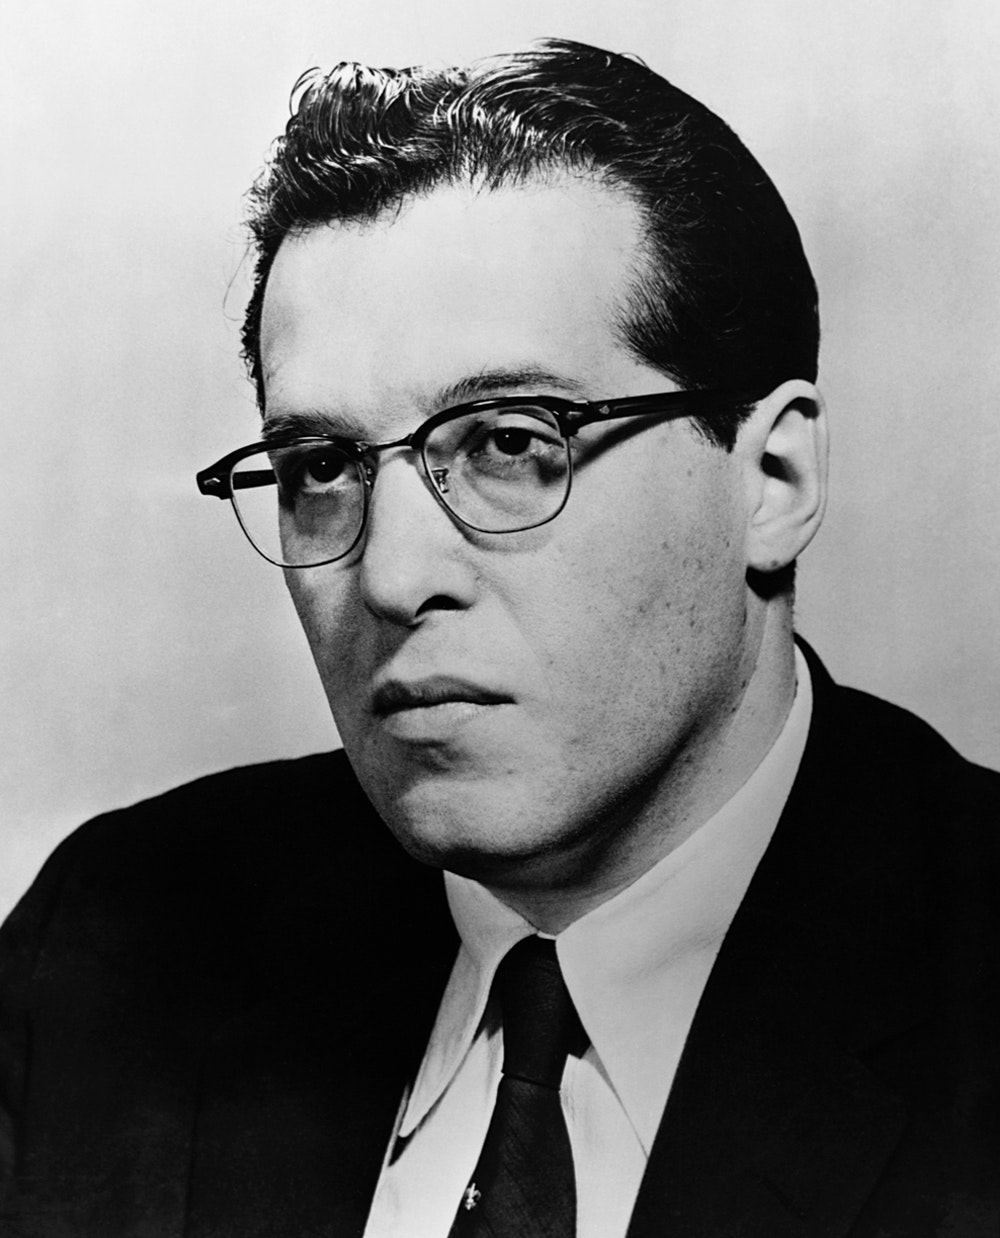
\includegraphics[scale=0.15]{images/schwinger.jpg}
	\end{subfigure}
	\begin{subfigure}{0.5\textwidth}
	\centering	
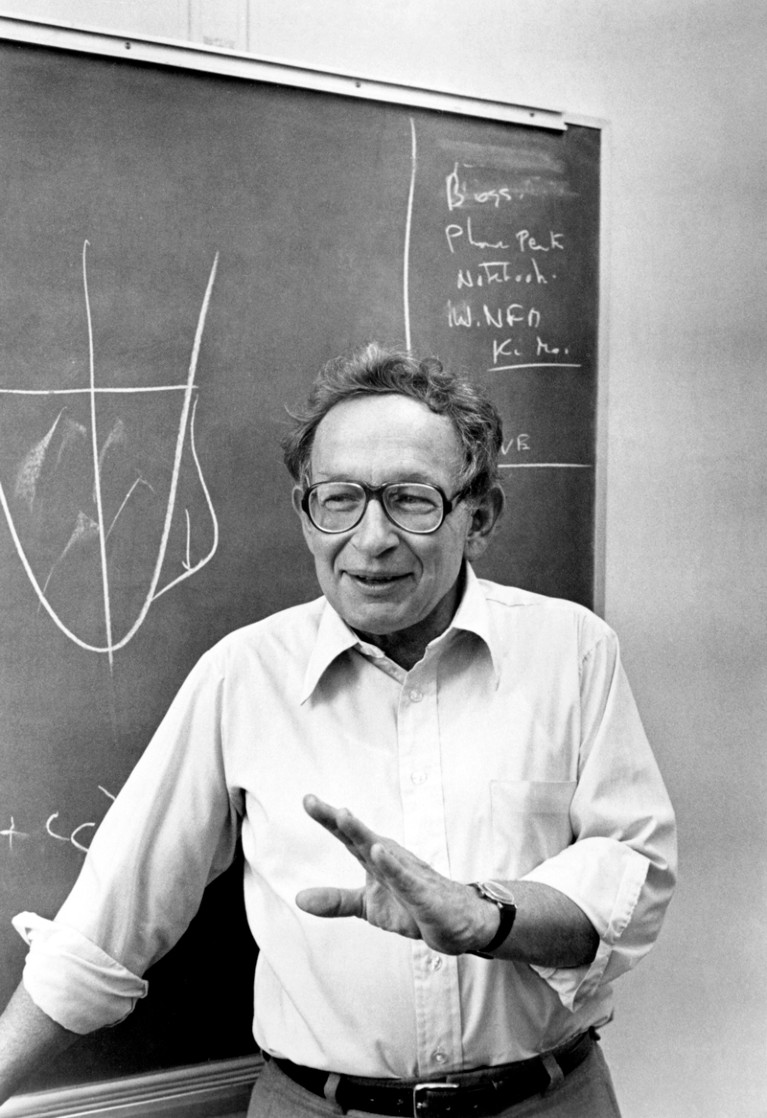
\includegraphics[trim = {1cm 1cm 4cm 12cm},clip,scale=0.25]{images/anderson.jpg}
		\end{subfigure}
\caption{Izquierda: Julian Schwinger, podemos trazar el descubrimiento
del mecanismo de Higgs a su trabajo pionero sobre c\'omo una simetr\'ia de norma no siempre implicaba un bos\'on de norma no masivo. Derecha: Philip Anderson descubri\'o el mecanismo que da
masa a los bosones de norma en el contexto de la superconductividad.}
	\end{figure}

\begin{figure}[h]
\centering
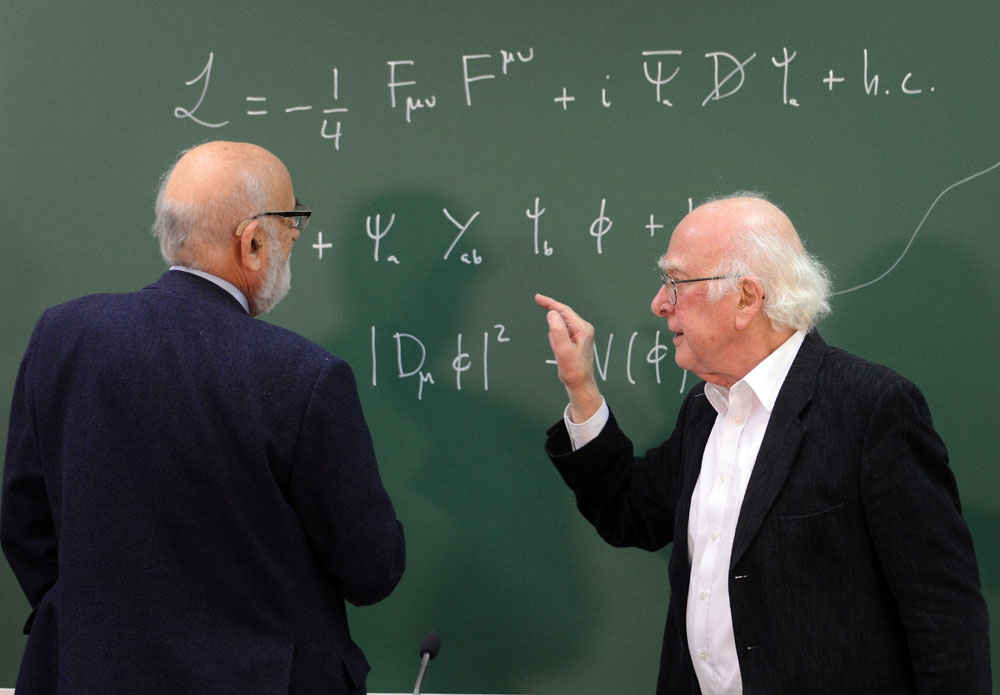
\includegraphics[scale=0.3]{images/higgs_englert_pizarra.jpeg}
\caption{Peter Higgs y Fran\c{c}ois Englert discutiendo el lagrangiano
que involucra al ahora llamado campo de Higgs, $\phi$.
?`Qu\'e creen que Higgs le dice a Englert? Tal vez le indique que
en la segunda l\'inea falta una barra en el campo fermi\'onico
$\bar \psi_a$.}
\end{figure}


Totalmente independientemente, en Mosc\'{u} en 1965, dos chicos de 19
a\~nos, ambos de nombre Alexander (o Sasha), con apellidos Migdal y
Polyakov, discutieron en gran detalle qu\'e significa el rompimiento
de una simetr\'ia \cite{Nobel13}. Ellos escribieron otro art\'iculo
parecido que fue publicado en 1966 \cite{MigPol}. Hace unos
a\~{n}os que Migdal visit\'o M\'exico y
% para un evento organizado por Alexander Turbiner, donde
relat\'o sobre las dificultades que ten\'{\i}an para publicar
este art\'iculo, ya qu\'e la comunidad de f\'{\i}sicos establecidos
en la Uni\'on Sovi\'etica -- bajo el liderazgo de Lev Landau -- rechaz\'o
la teor\'{\i}a cu\'antica de campos, que todav\'{\i}a era muy
controversial tambi\'en en el mundo occidental.\footnote{En Alemania
Werner Heisenberg era oponente influyente contra la teor\'ia cu\'antica
de campos; su preferencia era el formalismo de la matriz S.}
Finalmente, este art\'iculo
fue publicado algo tarde, pero despu\'es ambos Sashas se hicieron
famosos por otros trabajos --- en especial, Polyakov es conocido por
descubrir excitaciones topol\'ogicas que llamamos ahora instantones.

La explicaci\'on de c\'omo  las part\'iculas de norma -- y ciertas part\'iculas
acopladas -- pueden tener masa fue pronto conocida como el {\em mecanismo
de Higgs},\footnote{Consultar la literatura original no conduce a
  una explicaci\'on muy clara cu\'al es realmente la raz\'on por la que la
  terminolog\'ia excluye a Brout y Englert.}
  el tema de la Secci\'on 2 de este art\'iculo.
Su aplicaci\'on a la fenomenolog\'ia de part\'iculas elementales 
emergi\'o en 1967/8 por parte de Steven Weinberg \cite{Weinberg} y
Abdus Salam \cite{Salam}.
Ellos integraron este mecanismo al modelo de la interacci\'on
electrod\'ebil que Sheldon Glashow hab\'ia propuesto en 1961
\cite{Glashow} durante su estancia en Copenhague.
De hecho, Glashow estuvo presente en el seminario de Higgs en Harvard,
y reconoci\'o que era {\it ``a nice model''} \cite{boson}, pero no se le
occuri\'o la idea de que este mecanismo podr\'ia ser el remedio
para salvar a su modelo, que \'el ya hab\'ia abandonado.

Sin embargo, esta teor\'ia -- ahora conocida como el sector
electrod\'ebil del Modelo Est\'andar -- a\'un no era generalmente
aceptada ya que era considerada ``no renormalizable''.
En las teor\'ias cu\'anticas de campos casi siempre aparecen divergencias
a altas energ\'ias, as\'i que requieren una ``regularizaci\'on'',
una manipulaci\'on matem\'atica que convierte las divergencias
en un valores finitos. Se dice que una teor\'ia es {\em renormalizable}
si, al final del c\'alculo, se puede remover la regularizaci\'on
totalmente y llegar a predicciones finitas para las observables
(esta definici\'on es ligeramente simplista).

La comunidad f\'isica cambi\'o su punto de vista en 1971/2, gracias
al trabajo de Gerard 't Hooft, un brillante estudiante de doctorado
en Utrecht, Holanda, quien present\'o evidencia a favor de la
renormalizibilidad de dicho modelo (parcialmente junto a
su asesor, Martinus Veltman). Estos trabajos \cite{tHooft} fueron
una sensaci\'on que causaron un cambio de paradigma en aquella \'epoca.

\begin{figure}
\begin{subfigure}{0.5\textwidth}
	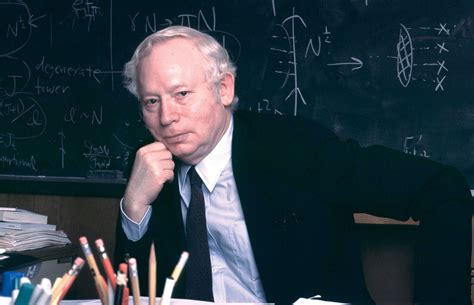
\includegraphics[scale=0.5]{images/weinberg.jpeg}
\end{subfigure}	
\begin{subfigure}{0.5\textwidth}
	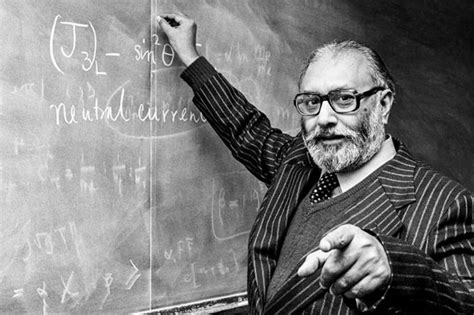
\includegraphics[scale=0.5]{images/salam.jpeg}
\end{subfigure}	
\caption{Steven Weinberg (izquierda) y Abdus Salam (derecha)
independientemente integraron el mecanismo de Higgs al sector
electrod\'ebil del Modelo Est\'andar.}
%Ambos compartieron el Premio
%Nobel de f\'isica en 1979 junto a Sheldon Glashow.}
\end{figure}

\begin{figure}
\centering
\begin{subfigure}{0.5\textwidth}
\centering
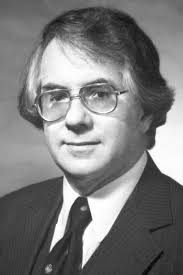
\includegraphics[scale=0.45]{images/glashow.jpeg}
\end{subfigure}\begin{subfigure}{0.5\textwidth}
\centering
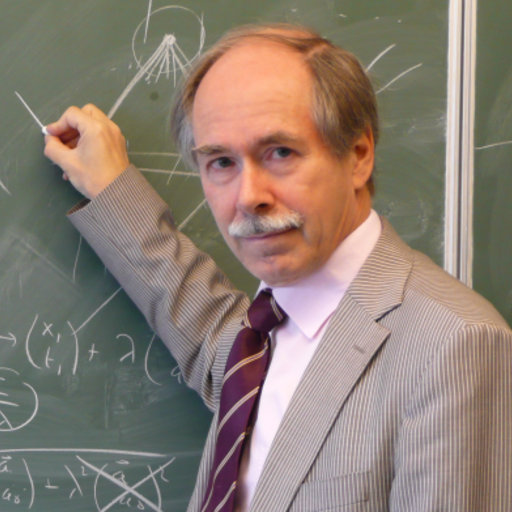
\includegraphics[scale=0.25]{images/thooft.jpg}
\end{subfigure}
\caption{Izquierda: Sheldon Glashow, creador de la versi\'on orignal
de la teor\'ia electrod\'ebil. Derecha: Gerard 't Hooft, famoso por
%fue galardonado
%con el Premio Nobel de f\'isca en 1999 debido a
su trabajo sobre la renormalizaci\'on del Modelo Est\'andar,
entre otras cosas.}
\end{figure}

La clave para este hito fue un nuevo m\'etodo, la {\em regularizaci\'on
dimensional} que est\'a entre los logros principales de la f\'isica en
Am\'erica Latina: fue propuesta primero por dos argentinos, Carlos Bollini
y Juan Jos\'e Giambiagi en 1971, aunque la publicaci\'on \cite{BolGiam}
se demor\'o hasta 1972. Ellos trabajaron en La Plata, en
circunstancias dif\'iciles durante la dictadura militar \cite{DimReg}.

Agregamos que hoy en d\'ia se da menos importancia a la pregunta
si el Modelo Est\'andar es renormalizable o no: la tendencia es que se
considera como teor\'ia efectiva, y su validez en un gran rango
energ\'etico -- que no tiene que extenderse hacia infinito --
es suficiente.

Poco despu\'es, en 1973, el Modelo Est\'andar de las part\'iculas
elementales fue completamente establecido, con un sector
electrod\'ebil \cite{Weinberg,Salam} y otro de la interacci\'on
fuerte \cite{QCD}. El mecanismo de Higgs es indispensable para
proporcionar masas a gran parte de las part\'iculas elementales.
Esto fue una revoluci\'on en la f\'isica de altas energ\'ias como no la
hemos visto m\'as en el medio siglo que sigui\'o, ya que despu\'es el
progreso fue relativamente lento.




En el siglo XXI es popular especular sobre f\'isica m\'as all\'a
del Modelo Est\'andar. Sin embargo, por ahora ninguna de estas propuestas
tiene apoyo s\'olido de datos experimentales. Por otro lado, los
experimentos han confirmado las predicciones del Modelo Est\'andar una
y otra vez: muchas veces salen al aire en las noticias que el
Modelo Est\'andar ha sido ``refutado''
por nuevos resultados, pero al final del an\'alisis, y la repetici\'on
de los experimentos, siempre sus predicciones han
triunfado.\footnote{Como ejemplo reciente, en la segunda parte de la
  d\'ecada pasada, se difundieron noticias de una tensi\'on entre el Modelo
  Est\'andar y experimentos con el decaimiento de mesones pesados
  conocidos como ``mesones B''. Al final, esta discrepacia no se
  substanci\'o. La \'ultima moda es el momento magn\'etico del
  mu\'on, donde el valor experimental parece un poquito diferente
  del c\'alculo basado en el Modelo Est\'andar. Si esto es verdad --
  cosa que no es nada segura -- la predicci\'on se equivoca al
  nivel relativo de $10^{-10}$: si lo comparamos con la distancia
  entre M\'exico y Europa central (Suiza por ejemplo), unos
  10,000\,km, esto corresponde a un posible error de la magntitud
  de mil\'imetros. Pero c\'alculos con simulaciones num\'ericas
  en la ret\'icula conducen a resultados m\'as cercanos al valor
  experimental, tendencia que indica que incluso esta discrepancia
  m\'inima podr\'ia desaparecer con un an\'alisis m\'as preciso,
  igual que todas las supuestas discrepancias anteriores.}
  
El Modelo Est\'andar es algo incompleto para describir al
universo (faltan por ejemplo la gravitaci\'on, materia oscura y
energ\'ia oscura), pero a\'un as\'i: se trata de nada menos que la
teor\'ia m\'as precisa y -- en este sentido -- m\'as exitosa en
la historia de la ciencia.\\
 
Higgs ya no particip\'o en este desarollo r\'apido. \'El ya era
tan famoso que pod\'ia permitirse casi no publicar m\'as resultados
de investigaci\'on a partir de la edad de 40 a\~{n}os.
(En M\'exico esto ser\'ia un problema serio con el SNII etc.)
 
Fue conocido como una persona tranquila y modesta, casi t\'imida,
que no busc\'o la atenci\'on medi\'atica o ponerse en el centro de
atenci\'on en eventos. Con su mentalidad de abstenerse del
{\it show,} se puede caracterizar como el contrario a Feynman.
Esta caracterizaci\'on corresponde a la impresi\'on de uno de los
autores (WB) qui\'en particip\'o en un congreso en Edimburgo 1997.
Higgs -- quien era em\'erito desde 1996 -- apareci\'o en el banquete,
pero muy discreto, simplemente para sentarse en una mesa sin
ning\'un espect\'aculo.

Esto no significa que Higgs no ten\'ia convicciones: fue
temporalmente activista por el desarmamento nuclear y
por el movimiento ambiental como miembro de {\it Greenpeace.}\\

Una vez que el Modelo Est\'andar hab\'ia sido establecido, su exploraci\'on
progres\'o con trabajo intenso en m\'ultiples pa\'ises.
En el a\~no 2000, todas sus part\'iculas ya eran experimentalmente
encontradas, menos una: la famosa ``part\'icula de Higgs'', involucrada
en este mecanismo, como vamos a describir en la Secci\'on 2.

Otra vez, la nomenclatura es tal vez un poco injusta con Englert y
Brout, pero as\'i es la convenci\'on de la comunidad.
Higgs no invent\'o este t\'ermino (esto lo hizo primero  Ben Lee
\cite{boson}), pero tambi\'en le era inc\'omodo el
apodo absurdo ``part\'icula de dios'' que no tiene ni el menor sentido.
Este t\'ermino fue propuesto por la editorial de un libro de divulgaci\'on
\cite{Lederman},
obviamente con un objetivo comercial, pero plenamente irresponsable.
Este t\'ermino se hizo popular y condujo a confusi\'on sin fin,
por ejemplo, la iglesia cat\'olica de Espa\~na crey\'o que el trabajo del
CERN tuviera algo que ver con teolog\'ia \cite{Guardian}. !`Tenemos que
tener cuidado con los t\'erminos que se usamos!

En el siglo XXI fuimos testigos de una carrera emocionante en la
b\'usqueda de la part\'icula de Higgs. En su fase final, era una
compentencia entre el Fermilab (cerca de Chicago) y el CERN
(cerca de Ginebra, sobre la frontera entre Suiza y Francia).
Despu\'es de primeras indicaciones en 2011, en 2012 las
colaboraciones ATLAS y CMS, ambos trabajando de manera independiente
en el Gran Colisionador de Hadrones (LHC) en el CERN, presentaron
evidencia indirecta pero clara de la observaci\'on de la
part\'icula de Higgs, que era tanto buscada \cite{ATLASCMS}.

	
\begin{figure}

\begin{subfigure}{0.5\textwidth}
	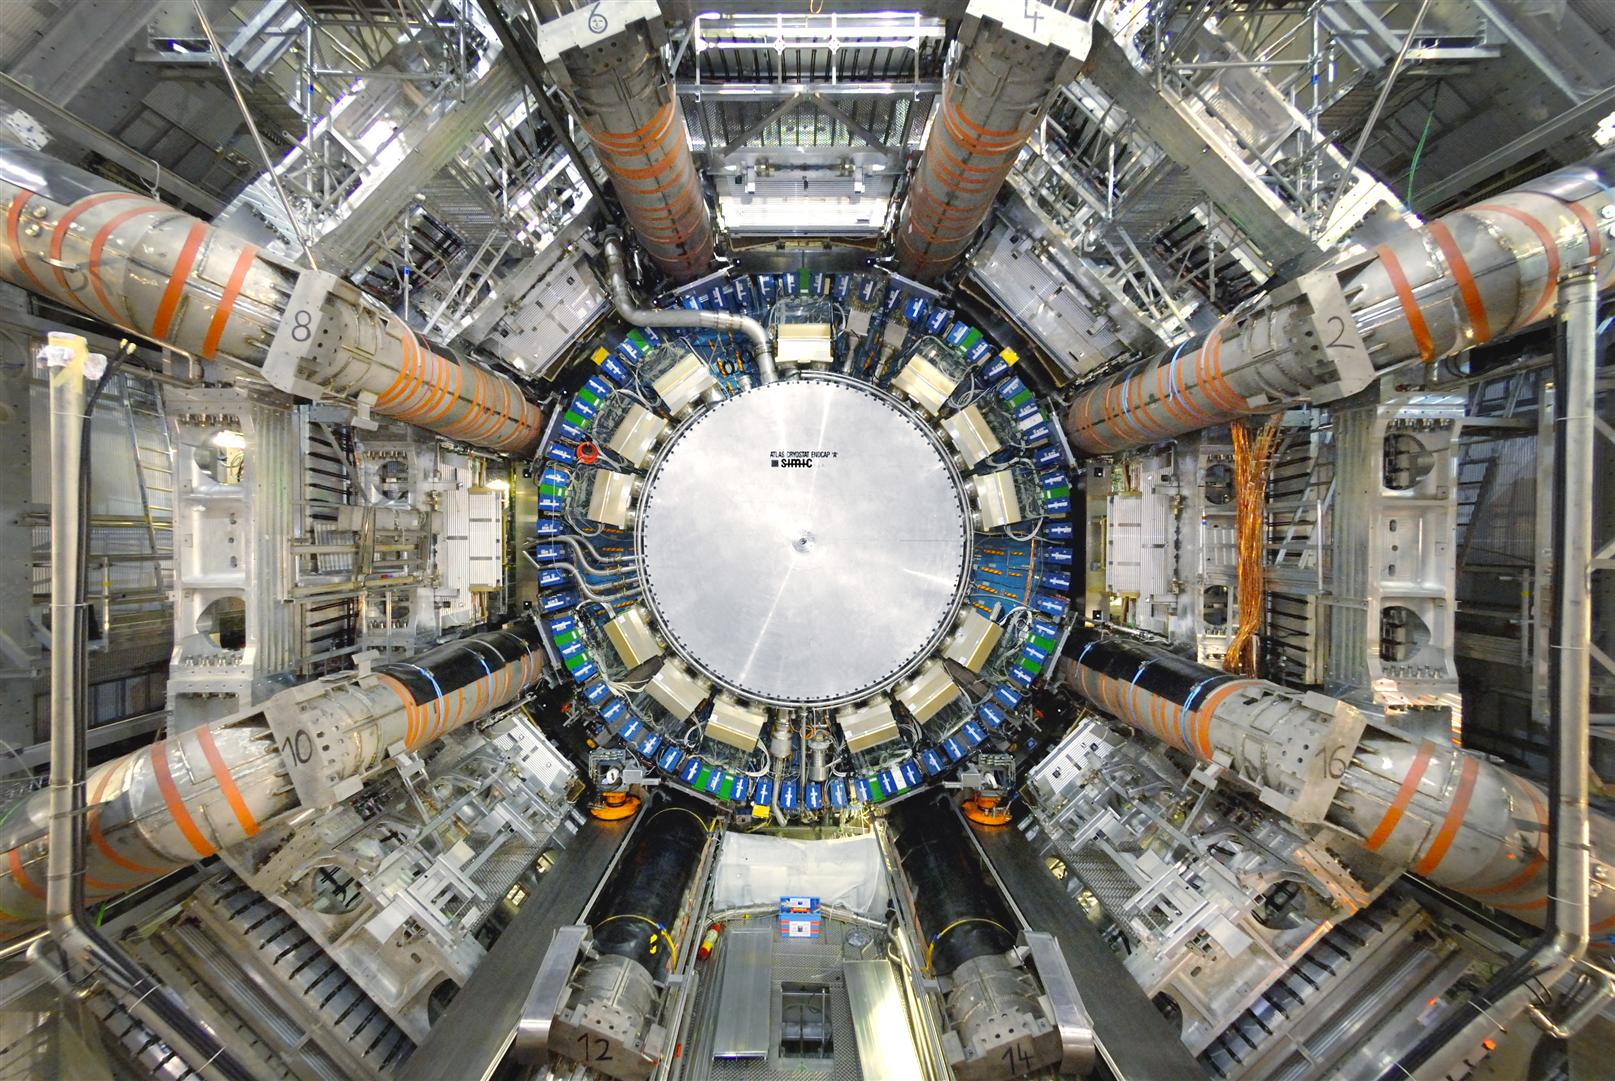
\includegraphics[scale=0.27]{images/atlas.jpg}
\end{subfigure}	
\begin{subfigure}{0.5\textwidth}
	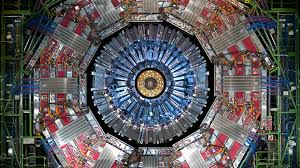
\includegraphics[scale=0.9]{images/cms.jpeg}
\end{subfigure}	
\caption{Detectores de la Colaboraci\'on ATLAS (izquierda) y CMS
(derecha) en el CERN que confirmaron las existencia del bos\'on
de Higgs del Modelo Est\'andar.
Ambos son detectores multiprop\'osito usados para
analizar colisiones entre part\'iculas de muy alta energ\'ia.}
\end{figure}


Con esto todo el conjunto de part\'iculas del Modelo Estandar
fue observado. As\'i se confirm\'o que el mecanismo de Higgs
est\'a realizado en la naturaleza, 48 a\~nos despu\'es de su
propuesta te\'orica. Esto se demor\'o casi el doble del tiempo
que la observaci\'on del neutrino (predicho por Wolfgang Pauli en 1930, y
detectado por Clyde Cowan, Frederick Reines y colaboradores en
1956),\footnote{Ref.\ \cite{neutrinos} revisa la historia y las
propiedades de los neutrinos, de una perspectiva semi-divulgativa.}
vemos que a veces vale la pena tener paciencia.

En particular, vali\'o la pena para Englert y Higgs, quienes recibieron
el Premio Nobel en 2013 por su predicci\'on correcta \cite{Nobel13};
tristemente, Brout hab\'ia muerto poco antes, en 2011.
En abril del 2024 nos lleg\'o la noticia del fallecimiento de Higgs,
a los 94 a\~nos, despu\'es de una breve enfermedad.

\begin{figure}
\centering
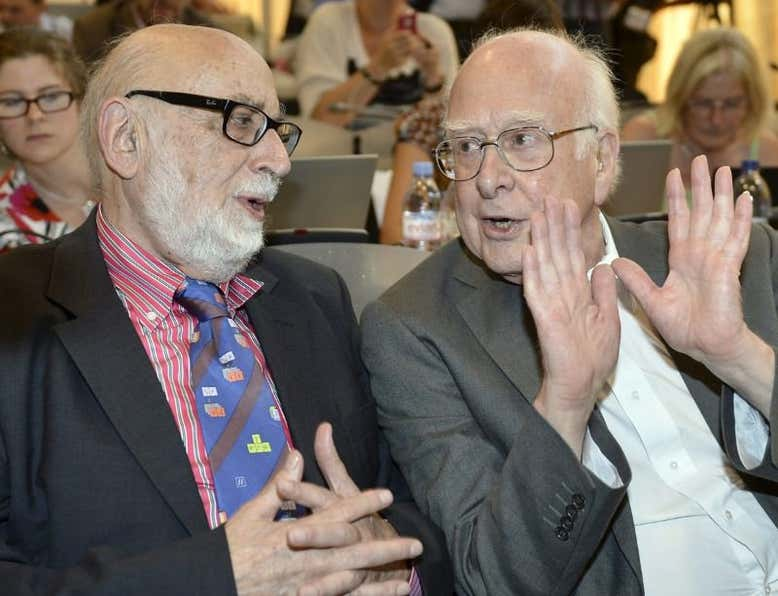
\includegraphics[scale=.3]{images/higgs_englert2.jpeg}
\caption{El 4 de julio de 2012 el CERN hizo p\'ublico el
descubrimiento del bos\'on de Higgs. Peter Higgs conmovido hasta
las l\'agrimas en la ceremonia dijo: ``Felicitaciones a todos los
involucrados en este descubrimento. Para m\'i es algo verdaderamente
incre\'ible que haya vivido para verlo''. La Real Academia Sueca de
las Ciencias otorg\'o el premio Nobel de F\'isica en 2013 a Fran\c{c}ois
Englert (izquierda) y a Peter Higgs (derecha) por ``el descubrimiento
te\'orico de un mecanismo que contribuye a nuestra comprensi\'on del
origen de la masa de las part\'iculas subat\'omicas $\dots$''
\cite{YouTube}.}
\end{figure}

\section{Mecanismo de Higgs}

Hasta donde sabemos, el mundo consiste de part\'iculas elementales, que
son indivisibles, y occurren en pocos tipos (decimos 25, pero depende
un poco de como se cuenta). Ejemplos famosos son el electr\'on y el
fot\'on (la part\'icula de la luz).

Su descripci\'on relativista funciona con ``campos'', objetos
abstractos, presentes en todo el universo, en cualquier momento.
En un punto, un campo puede tomar diferentes estados, que dependen
del tiempo. Si los campos en una regi\'on est\'an en su estado base,
percibimos el vac\'io. Las excitaciones son cu\'antizadas y se
manifiestan como part\'iculas elementales -- esto es la idea de la
{\it teor\'ia cu\'antica de campos.}

Existe un campo para cada tipo de part\'icula elemental,
y sus excitaciones pueden moverse (como ondas), interactuar,
generar y destruir part\'iculas (esto es un requisito para
la compatibilidad con la Relatividad Especial, que falta en
la mec\'anica cu\'antica).\footnote{Ref. \cite{WBparti} presenta
  otra explicaci\'on divulgativa pero m\'as extensa.}

Un concepto central son las simetr\'ias: una simetr\'ia significa
la invarianza de las propiedades f\'isicas bajo un grupo de
transformaciones de uno o varios campos. Distinguimos simetr\'ias
{\em globales} y {\em locales:}

\begin{itemize}

\item En una simetr\'ia {\em global,} un campo se transforma de la
  misma manera en todas partes. Se puede imaginar un grupo de personas
  que hacen gimnasia colectiva, todas hacen el mismo movimiento,
  puede ser sincronizado con m\'usica.
  (La imagen es un poco simplista porque los campos se transforman
  de la misma manera incluso en todo el espacio-tiempo.)
  
\item El caso de una simetr\'ia {\em local} se puede imaginar como
  gimnasia ca\'otica: cada persona se mueve como quiere, de manera
  independiente. Esto significa que los campos pueden ser transformados
  independientemente en cada punto del espacio-tiempo.

  Es claro que este tipo de simetr\'ia permite muchas m\'as
  transformaciones.
  Lograr una simetr\'ia local es m\'as dif\'icil, pero conduce
  a restricciones m\'as fuertes, y por lo tanto a una poderosa
  capacidad de hacer predicciones.
  
  T\'ecnicamente, se introduce un campo adicional, conocido como
  ``campo de norma'', que transforma tal que compensa el cambio
  relativo entre puntos cercanos en una transformaci\'on simult\'anea.
  Este concepto exitoso describe la transmisi\'on de interacciones,
  pero solamente funciona si la simetr\'ia local es exacta.
  
\end{itemize}

Una categor\'ia importante de part\'iculas es conocida como
``fermiones'': los fermiones elementales (conocidos) tienen
``esp\'in $1/2 $'' en unidades naturales.\footnote{Para
usar unidades naturales, se coloca la constante
cu\'antica de Planck y la velocidad de la luz en el vac\'io a 1,
$\hbar = c =1$.}
El esp\'in es un grado de libertad interno que se manifesta como
momento angular. Ejemplos para fermiones son el electr\'on, sus dos
``primos'' m\'as pesados (el mu\'on y el tau\'on), los neutrinos (mucho
m\'as ligeros y sin carga el\'ectrica)\footnote{El conjunto del
electr\'on, mu\'on, tau\'on y los tres neutrinos es conocido como
los {\em leptones}.}
y los cuarks (constituyentes
de part\'iculas compuestas, como el prot\'on y el neutr\'on).

Un fermi\'on puede existir en dos variantes, con ``quiralidad''
izquierda o derecha; se pude imaginar como manos,\footnote{Efectivamente,
el t\'ermino viene de ``kheir'', que significa ``mano'' en griego.} 
o guantes, izquierdo o derecho, pero en un sentido abstracto.

Suponemos por ejemplo un electr\'{o}n sin masa: en este caso,
el electr\'on izquierdo ($e_L$) y derecho ($e_R$) son independientes,
y su esp\'in apunta contra (para $e_L$) o en (para $e_R$) la
direcci\'on de su movimiento (una part\'icula sin masa no
puede estar en reposo). Esto es ilustrado simbolicamente en
la Figura \ref{electron}.

\begin{figure}
\centering
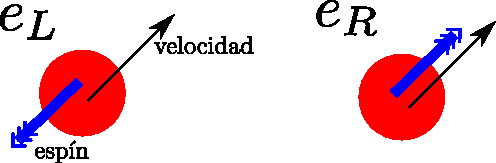
\includegraphics[scale=1]{images/quiral.pdf}
\caption{Representaci\' on simb\'olica de un electr\'on sin masa con
quiralidad izquierda $e_L$ (izquierda) y quiralidad derecha $e_R$
(derecha). La direcci\'on del movimiento es
indicada por la flecha delgada y la direcci\'on del esp\'in
por la flecha gruesa. Para quiralidad izquierda velocidad y
esp\'in apuntan en direcciones contrarias, pero para la quiralidad
derecha apuntan en la misma direcci\'on.}
\label{electron}
\end{figure}
Incluir un t\'ermino de masa requiere de un producto de los campos
del electr\'on izquierdo y derecho (se puede imaginar que las dos
manos se agarran). Entonces ya no son independientes, y bajo una
simetr\'ia tienen que transformarse de la misma manera.

Sin embargo, esto no es el caso en la teor\'ia electrod\'ebil de Glashow
\cite{Glashow}: esta teor\'ia permite, por ejemplo, transformaciones
locales (``de norma'') que solamente afectan al $e_L$, pero no al $e_R$.
Aqu\'i era el problema: dicha teor\'ia pareci\'o ser incompatible con
el t\'ermino de masa del electr\'on (y de otros fermiones), pero sabemos
que el electron s\'i tiene una masa de $M_e \simeq 0.511\ {\rm MeV}$
(todav\'ia en unidades naturales).

De hecho, la situaci\'on era a\'un peor. Las part\'iculas de norma
que transmiten la fuerza d\'ebil se llaman $W^{\pm}$, $Z^0$
(con carga el\'ectrica $\pm1, \, 0$), por ejemplo los $W$ son
responsables del decaimiento radioactivo. Esta fuerza tiene un
alcance muy corto (como $10^{-17}$~m) que solamente se puede
explicar si $W^{\pm}$, $Z^0$ tienen masas grandes (est\'an entre
las part\'iculas elementales m\'as pesadas que conocemos, con
masas de $M_W = 80.4 \, {\rm GeV}$ y $M_Z = 91.2\,{\rm GeV}$). 
Pero igual que la masa del electr\'on, parece que la simetr\'ia
de norma -- que tiene que ser exacta -- requiere $m_W = m_Z = 0$.

El acertijo de d\'onde pueden venir estas masas de part\'iculas
de norma era una ``pregunta matadora'' con la cual Wolfgang Pauli
destruy\'o un seminario de Chen-Ning Yang en Princeton en 1953
sobre teor\'ias de
norma con un grupo de simetr\'ia no abeliano (ahora conocidas como
teor\'ias de Yang-Mills). Sin conocer el mecanismo de Higgs, Yang no
logr\'o contestar, pero Pauli insisti\'o tanto hasta
que Yang se sent\'o frustrado. Finalmente Robert Oppenheimer tuvo
que animarlo para continuar su charla \cite{Shifman}.

Entonces, ?`c\'omo funciona la salvaci\'on de esta teor\'ia,
el mecanismo de Higgs? Primero, se agrega otro campo m\'as,
el {\em campo de Higgs}, usamos la notaci\'on $\phi (x)$.
La variable $x$ es un punto del espacio-tiempo, y $\phi$ es
un campo escalar, sus fluctuaciones representan part\'iculas 
con esp\'in 0. Para establecer un t\'ermino de masa del electr\'on,
ahora se forma un producto de {\em tres} campos, $e_L$, $\phi$ y
$e_R$.\footnote{Realmente necesitamos parcialmente anti-campos,
que representan anti-part\'iculas, pero ignoramos
este aspecto en el contexto de este art\'iculo de divulgaci\'on.}
El campo de Higgs tambi\'en transforma bajo la simetr\'ia local,
de tal manera que el t\'ermino en su totalidad s\'i es invariante
de norma.

Entonces de esta manera se puede agregar un t\'ermino permitido
(invariante de norma), pero ?`esto proporciona una masa al electr\'on?
Posiblemente s\'i, puede funcionar con el escenario siguiente.

A bajas energ\'ias, el campo de Higgs ``se congela'' en su estado
base, se manifiesta casi como una constante. Esta constante no
tiene que ser cero: realmente $\phi$ tiene 4 componentes reales, pero
nos podemos imaginar que sean 2 solamente,
$\phi_1 , \, \phi_2 \in \R$, que parametrizan un plano.
Este campo viene con un potencial $V(\phi_1, \phi_2)$ de la forma
de un sombrero, con el valor cero al centro, pero hay un anillo
de m\'inimos que corresponden a un valor
$|\phi|^2 = \phi_1^2 + \phi_2^2 > 0$, como est\'a ilustrado en la
Figura \ref{sombrero}.
Este ``valor esperado en el vac\'io'' toma el papel de la masa
del electr\'on que el modelo necesita (hasta un coeficiente),
$M_e \propto |\phi|$, y de manera an\'aloga tambi\'en se obtienen
las masas $M_W$ y $M_Z$, todos conforme a la simetr\'ia de norma
(regresaremos a este tema).

Parece todo bien, pero hay otro problema todav\'ia, y a esto
Coleman se refiri\'o en su comentario sobre el seminario de
Higgs en Harvard, que hemos mencionado en Secci\'on 1.

El potencial sombrero tiene una simetr\'ia bajo rotaciones por
el centro. Suponemos que el campo $\phi$ elige uno de
los m\'inimos: el proceso de esta elecci\'on se denota como
``rompimiento espont\'aneo de la simetr\'ia'': desde
la perspectiva de un m\'inimo espec\'ifico, ya no se ve la
simetr\'ia de rotaci\'on. En Ref.\ \cite{HiggsBol} hemos
descrito este proceso con la analog\'ia del {\em Asno de Buridan,}
que est\'a sediento y rodeado por un abrevadero de agua, pero
tiene que decidirse en que direcci\'on camina para beber agua.

Peque\~nas fluctuaciones del campo m\'as all\'a de su estado
m\'inimo corresponden a part\'iculas. Si una fluctuacion es
{\em radial,} cuesta energ\'ia porque el potencial sube -- esto
es una part\'icula masiva (la curvatura del potencial en la
direcci\'on radial corresponde a la masa en cuadrado.)
Por otro lado, una fluctuaci\'on {\em tangencial} no necesita
energ\'ia, pues el campo se queda con energ\'ia m\'inima.
Esto es un ejemplo de una part\'icula sin masa, conocido
como un {\em bos\'on de Nambu-Goldstone} \cite{Nambu,Goldstone}.
Seg\'un el Teorema de Goldstone \cite{GSW}, estos bosones aparecen
cuando una simetr\'a continua (como la rotaci\'on en este
ejemplo) se rompe espont\'aneamente.

Si el mecanismo funciona como descrito antes, se queda la
pregunta: ?`d\'onde est\'a este bos\'on de Nambu-Goldstone?
Por ser sin masa, tendr\'a que tomar un papel importante
y dominar la f\'isica a bajas energ\'ias (donde part\'iculas
muy pesadas no se manifiestan). Pero ninguna part\'icula de
este estilo fue observada. Entonces para justificar el mecanismo,
se tiene que ``evadir el Teorema de Goldstone'', como dijo
Coleman, y sus colegas en Harvard dudaron si esto es posible.
No eran los \'unicos, por ejemplo Klaus Hepp, prominente
f\'isico matem\'atico, advirti\'o a Higgs que esto no podr\'ia
funcionar porque el Teorema estaba demostrado con \'algebra
C$^{*}$, un formalismo que Higgs no conoc\'ia, pero \'el expres\'o
sus dudas de las suposiciones en esta demostraci\'on \cite{boson}.

Ahora sabemos que el teorema s\'i es correcto, pero solamente
se refiere al rompimiento de una simetr\'ia cont\'inua
{\em global} -- esta suposici\'on estaba escondida.
La observaci\'on crucial era que la situaci\'on es diferente
en el caso de una simetr\'ia {\em local}: en este caso, los
m\'inimos est\'an conectados por transformaciones locales, o
transformaciones de norma, por lo tanto f\'isicamente id\'enticas.
As\'i no hay fluctuaciones f\'isicas entre los m\'inimos, y no hay
bosones de Nambu-Goldstone. Lo que pasa, y completa el mecanismo
de Higgs, es que el bos\'on de norma adquiere masa, lo que significa
que el grado de libertad que ten\'ia el boson de Nambu-Goldstone
se convierte en un grado de libertad longitudinal del bos\'on de
norma (sin masa solamente tiene grados de libertad transversales).
En lenguaje popular, se dice que el bos\'on de norma ``se come''
el bos\'on de Nambu-Goldstone: este \'ultimo ya no est\'a, pero
el primero se hace ``gordo''.

Esto hab\'ia observado Anderson antes en un t\'ipico superconductor:
en su interior, a muy baja temperatura, el fot\'on adquiere masa,
por esto casi no puede penetrar el superconductor -- un fen\'omeno
conocido como {\em efecto de Meissner-Ochsenfeld.}
Brout, Englert y Higgs extendieron este efecto a modelos
relativistas \cite{EB,Higgs}, y Weinberg y Salam a la fenomenolog\'ia
de la interacci\'on electrod\'ebil \cite{Weinberg,Salam}.
Hemos mencionado que el campo de
Higgs tiene 4 componentes reales: siempre hay una fluctuaci\'on
masiva radial, y entonces 3 bosones de Nambu-Goldstone si tratamos
con una simetr\'ia global. Cuando la promovemos a una simetr\'ia
local, los bosones $W^+$, $W^-$ y $Z^0$ ``se comen'' estos
bosones de Nambu-Goldstone y adquieren masas,
mientras que el fot\'on se queda sin masa (en circunstancias
normales) y describe el electromagnetismo que tiene alcance largo.

\begin{figure}
\vspace*{-5mm}
	\begin{center}
	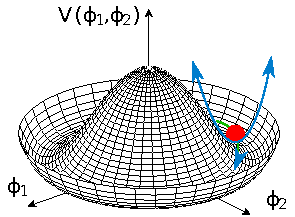
\includegraphics[scale=2]{images/higgspotential.pdf}
	\end{center}
	\caption{Potencial de Higgs: desde la perspectiva de la
        cima el potencial es sim\'etrico de rotaci\'on.
        Sin embargo, desde la perspectiva de la bola el potencial
        parece no presentar dicha simetr\'ia, esto es el ``rompimiento
        espont\'aneo de simetr\'ia''. Las fluctuaciones {\em tangenciales}
        del campo a lo largo del c\'irculo de m\'inimos se manifiestan
        como un bos\'on de Nambu-Goldstone si la simetr\'ia es global.
        Si la simetr\'ia es local, este bos\'on de Nambu-Goldstone
        est\'a ``comido'' por un campo de norma que adquiere masa. Las
        fluctuaciones {\em radiales}, perpendiculares al c\'irculo de
        m\'inimos, se manifiestan como una part\'icula masiva. Si
        tratamos con el potencial de Higgs como ocurre en el Modelo
        Est\'andar, esta part\'icula masiva es el famoso bos\'on de
        Higgs.}
\label{sombrero}        
\vspace*{-2mm}
\end{figure}

Ya hemos visto que el mecanismo tambi\'en proporciona una masa al
electr\'on, y de la misma manera aplica al mu\'on, tau\'on y a
todos los cuarks. ?`Y qu\'e pasa con el campo de Higgs?
Sabemos que 3 de sus 4 componentes ser\'ian bosones de
Nambu-Goldstone que desaparecen, pero est\'a la cuarta componente
todav\'ia, que corresponde a la fluctuaci\'on radial, es decir,
a una part\'icula masiva. Su existencia es una predicci\'on del
mecanismo de Higgs, y en este aspecto el segundo art\'iculo de Higgs
de 1964 era algo m\'as expl\'icito que los otros trabajos originales.
Esto era en el contexto de modelos juguete todav\'ia, pero una vez se
aplic\'o a un modelo fenomenol\'ogico, se concluy\'o que dicha
{\em part\'icula de Higgs} tendr\'ia que ser observable. 

La teor\'ia no predice la masa de la part\'icula de Higgs, $M_{\rm H}$
(se pueden derivar cuotas solamente que eran tema de discusi\'on durante
muchos a\~nos), por lo que la b\'usqueda experimental era dif\'icil.
Al inicio del siglo XXI, los experimentos del
Gran Colisionador de Leptones y Protones (LEP) del CERN demostraron
que tiene que tener una masa de $M_{\rm H} > 114\, {\rm GeV}$. Entonces se
sab\'ia que tiene que ser muy pesado (si existe), tal que su creaci\'on
requiere colisiones de altas energ\'ias. Esto tambi\'en implica que
su tiempo de vida es muy corto, decae en promedio en $10^{-22}$
segundos, y no puede dejar trazas en ning\'un detector.

Un experimento tiene que capturar los productos de su decaimiento
que permiten la reconstrucci\'on de la part\'icula de Higgs como
estado intermediario, o ``resonancia'' -- por muy poco tiempo --
en una colisi\'on a
altas energ\'ias. El an\'alisis de las part\'iculas que resultan al
final del proceso permiten reconstruir las propiedades de la
part\'icula de Higgs, en particular su masa de $M_{\rm H} = 125\,
{\rm GeV}$ y su esp\'in 0, que confirma que se trata de una part\'icula
escalar.

En el canal m\'as limpio que fue observado, el decaimiento del la
part\'icula de Higgs termina con dos fotones, un estado final que
no ser\'ia posible si, por ejemplo, la part\'icula original
ten\'ia esp\'in 1, como Landau hab\'ia demostrado \cite{Landau}.
Pero los experimentos ATLAS y CMS estudiaron (independientemente)
muchos m\'as decaimientos en gran detalle -- como, por ejemplo,
con un estado final de cuatro leptones -- y no dejan ninguna duda
de la existencia de la part\'icula de Higgs, y del mecanismo
correspondiente.


\begin{figure}
\centering
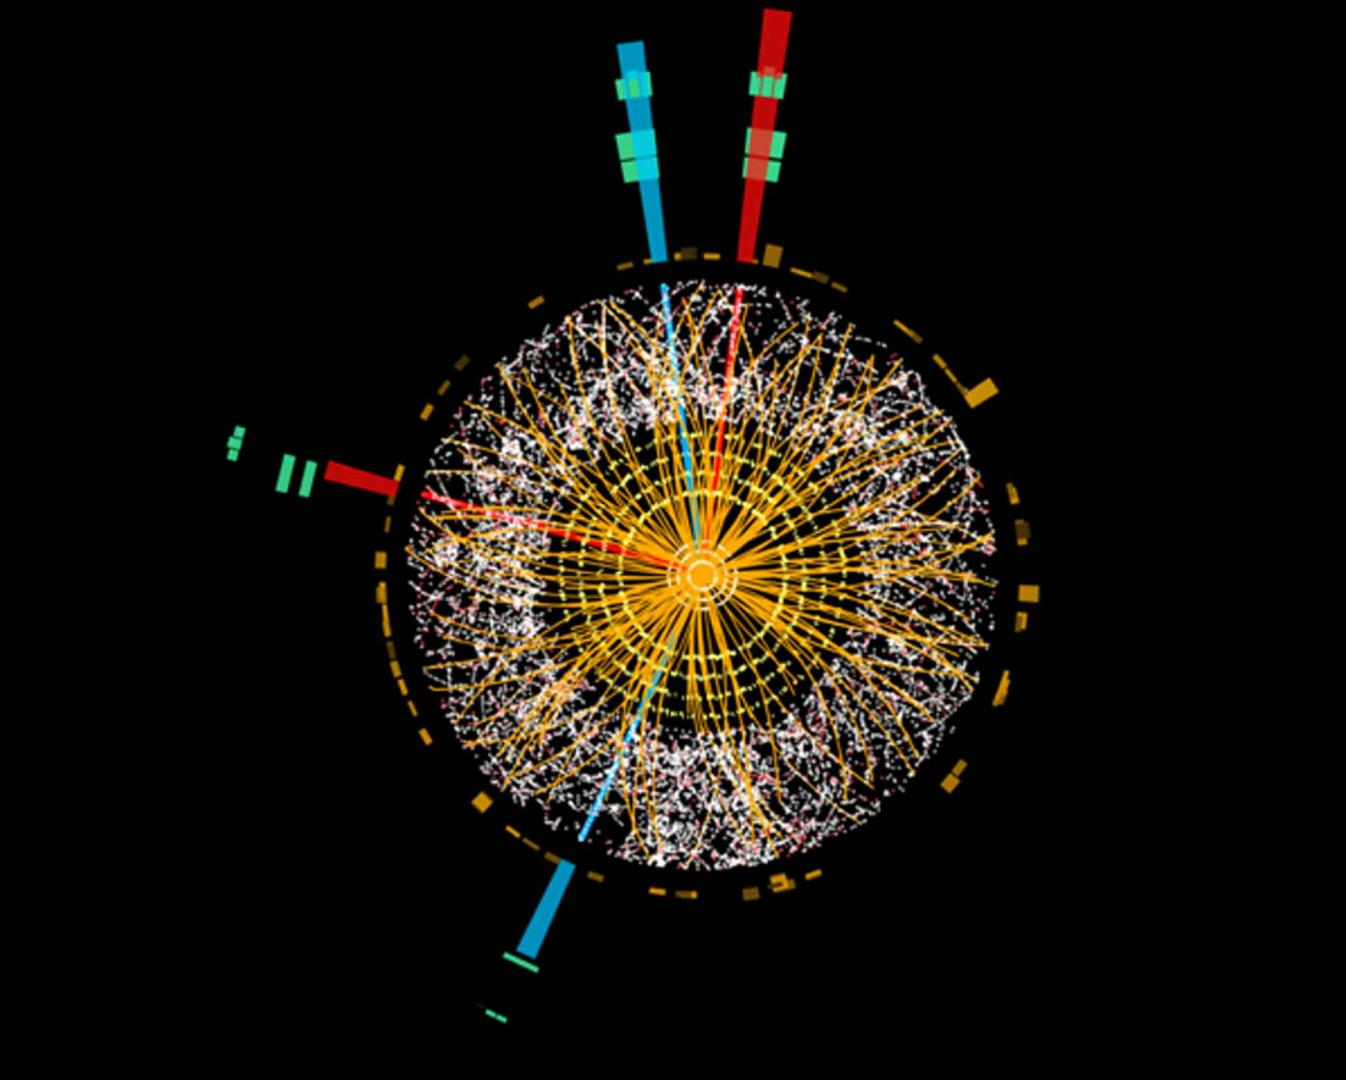
\includegraphics[scale=0.2]{images/atlas-higgs.jpg}
\caption{Canales posibles del decaimiento del bos\'on de
Higgs es cuando decae a dos bosones $Z$ que a su vez decaen cada
uno en un par lepton-antilepton. 
En la imagen observamos 4 leptones (l\'ineas rojas y azules) que
posiblemente hayan sido producidas por el decaimiento del bos\'on de Higgs.}
\end{figure}

\begin{figure}
\centering
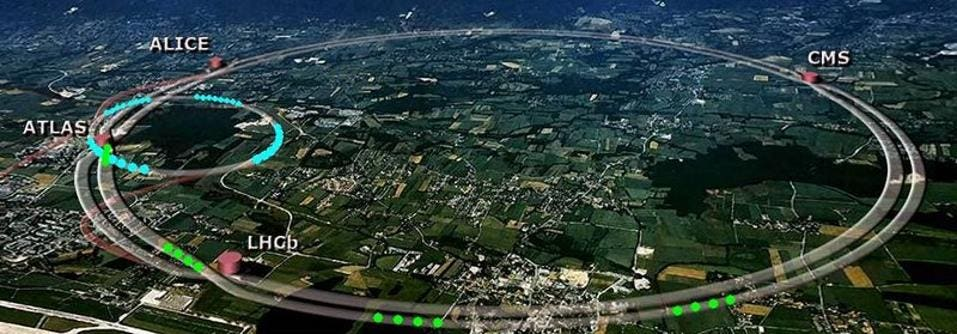
\includegraphics[scale=0.4]{images/lhc.jpg}
\caption{El Gran Colisionador de Hadrones (LHC por sus siglas en
ingl\'es) se encuentra ubicado en la regi\'on fronteriza entre
Francia y Suiza.
Sus cuatro experimentos principales se llaman ATLAS y CMS (que
de manera independiente encontraron evidencia de la existencia
del bos\'on de Higgs), ALICE (con fuerte participaci\'on mexicana)
y LHCb.}
\end{figure}

Esto representa un \'exito espectacular de la f\'isica de part\'iculas
elementales. A\'un as\'i, no todo est\'a resuelto todav\'ia. Desde la
perspectiva conceptual, se queda el {\em problema de la jerarqu\'ia}
y respecto a la fenomenolog\'ia, el mecanismo de Higgs no explica
el origen de todas las masas que obervamos. Terminamos con
comentarios breves sobre estos asuntos:

\begin{itemize}

\item {\em Problema de la jerarqu\'ia:} Si empezamos con un sistema
cl\'asico (sin efectos cu\'anticos) y suponemos una masa $m_{\rm H}^{(0)}$
en la magnitud de las masas de otras part\'iculas,
es natural que las correcciones cu\'anticas suben dicha masa
dr\'asticamente, a un valor $m_{\rm H}$ del orden de la ``escala de
Planck'' (determinada por la constante de la gravitaci\'on).
Pero esto conduce a un valor de $m_{\rm H}$ muy alto, t\'ipicamente
como $10^{17}$ veces su valor observado.

Lo que se podr\'ia hacer es suponer un valor de $m_{\rm H}^{(0)}$
extremadamente negativo, as\'i que el efecto cu\'antico
se cancela casi totalmente, y se queda un resto diminuto
de 125\,GeV. Pero esta aproximaci\'on -- con una cancelaci\'on
entre dos contribuciones tremendas que deja un resto diminuto --
no parece natural. Esto es conocido como el ``problema de la
jerarqu\'ia''. Sin embargo, no es una paradoja, se puede llegar
de manera consistente a 125\,GeV, y la pregunta de qu\'e tan
grave es este problema es un poco filos\'ofica.

\item Los {\em neutrinos} (descritos con el s\'imbolo $\nu$) tienen
un papel especial: en la forma tradicional del Modelo
Est\'andar se supuso que ten\'ian masa cero, $M_{\nu} =0$,
y que solamente exist\'ia el neutrino con quiralidad izquierda,
$\nu_L$.

Esto es consistente en teor\'ia, pero a finales del siglo XX
se observ\'o que los neutrinos s\'i tienen una peque\~na masa,
$m_{\nu}>0$ -- repetimos que Ref.\ \cite{neutrinos} presenta una
revisi\'on semi-divulgativa del tema.

De primera vista, conforme con nuestra descripci\'on anterior,
parece inevitable que exista el neutrino derecho, $\nu_R$.  
Esto permite la aplicaci\'on del mecanismo de Higgs para los
neutrinos, y adem\'as otro tipo de masa, solamente para el
$\nu_R$, conocido como ``masa de Majorana''.

Sin embargo, el $\nu_R$ no es observado, y su existencia no
es realmente inevitable: podemos construir una t\'ermino de masa
que involucra \'unicamente el campo $\nu_L$. Este t\'ermino no
es renormalizable, pero hemos mencionado en la Secci\'on 1 que ya no
se da tanta importancia a esta propiedad. Entonces este escenario
ser\'ia la alternativa, en el marco del Modelo Est\'andar interpretado
como teor\'ia efectiva que funciona en cierto rango energ\'etico.

\item Hasta este punto, el mecanismo de Higgs explica las masas
de las part\'iculas elementales (con la posible excepci\'on de
los neutrinos), y hay otras part\'iculas como el fot\'on que se
quedan sin masa. Parece una imagen completa del origen de la masa.

Sin embargo, el mundo real es diferente: en realidad, la masa de un
objeto macrosc\'opico de nuestra vida cotidiana viene solamente
por $1 \dots 2 \, \%$ del mecanismo de Higgs, que conduce a las
masas de las cuarks.

Estas masas cotidianas consisten principalmente de masas de
nucleones (protones y neutrones) que de su parte consisten
esencialmente de energ\'ia de {\em gluones} (otras part\'iculas de
norma, que transmiten la interacci\'on fuerte): tienen masa cero,
pero son confinados al interior de un nucle\'on (u otra part\'icula
compuesta por la interacci\'on fuerte). Su energ\'ia se
manifiesta como casi toda la masa del nucle\'on, mientras que
las masas da los cuarks solamente proporcionan dicha contribuci\'on
al nivel de $\sim 1 \dots 2 \, \%$.

El interior de un nucle\'on es un sistema muy, pero muy complejo,
por mucho tiempo pareci\'o imposible calcular algo conclusivo
al respecto. Sin embargo, hace un poco m\'as de una d\'ecada 
se logr\'o calcular por ejemplo la masa del nucle\'on,
$M_N \simeq 939\,{\rm MeV}$, de primeros principios, hasta una
incertidumbre del orden de 1\,\%. Este c\'alculo captura
el despelote hiper complicado de gluones (y ``cuarks de mar'',
parejas inestables de un cuark y su anti-cuark), y el
resultado es compatible con los experimentos. La pregunta de
c\'omo estos c\'alculos eran posibles ser\'ia tema para otro
art\'iculo $\dots$

\end{itemize}

\begin{thebibliography}{10}

\bibitem{Higgs} P.W.\ Higgs,
% Broken symmetries, massless particles and gauge fields,
{\em Phys.\ Lett.}\ {\bf 12} (1964) 132-133;
% doi:10.1016/0031-9163(64)91136-9
% Broken Symmetries and the Masses of Gauge Bosons,
{\em Phys.\ Rev.\ Lett.}\ {\bf 13} (1964) 508-509.
% doi:10.1103/PhysRevLett.13.508
% Spontaneous Symmetry Breakdown without Massless Bosons,
{\em Phys.\ Rev.}\ {\bf 145} (1966) 1156-1163.
% doi:10.1103/PhysRev.145.1156

\bibitem{boson} P.\ Higgs,
% My Life as a Boson: The Story of ``The Higgs'',
{\em Int.\ J.\ Phys.}\ {\bf A17} (2002) 86-88.
% https://doi.org/10.1142/S0217751X02013046

\bibitem{EB} F.\ Englert y R.\ Brout,
% Broken Symmetry and the Mass of Gauge Vector Mesons,
{\em Phys.\ Rev.\ Lett.}\ {\bf 13} (1964) 321-323.
% doi:10.1103/PhysRevLett.13.321

\bibitem{GHK} G.S.\ Guralnik, C.R.\ Hagen y T.W.B.\ Kibble,
% Global Conservation Laws and Massless Particles,
{\em Phys.\ Rev.\ Lett.}\ {\bf 13} (1964) 585-587.
% doi:10.1103/PhysRevLett.13.585

\bibitem{Anderson} P.W.\ Anderson,
% Plasmons, Gauge Invariance, and Mass,
{\it Phys.\ Rev.}\ {\bf 130} (1963) 439-442.
% doi:10.1103/PhysRev.130.439

\bibitem{Schwinger} J.S.\ Schwinger,
% Gauge Invariance and Mass,
  {\em Phys.\ Rev.}\ {\bf 125} (1962) 397-398;
% doi:10.1103/PhysRev.125.397
% Gauge Invariance and Mass. 2.,
{\em Phys.\ Rev.}\ {\bf 128} (1962) 2425-2429.
% doi:10.1103/PhysRev.128.2425

\bibitem{Nobel13} Royal Swedish Academy of Sciences,
  ``Scientific Background: The BEH-Mechanism, Interactions with Short
  Range Forces and Scalar Particles'',\\
  www.nobelprize.org/prizes/physics/2013/advanced-information/
  
\bibitem{MigPol} A.A.\ Migdal y A.M.\ Polyakov,
% SPONTANEOUS BREAKDOWN OF STRONG INTERACTION SYMMETRY
% AND THE ABSENCE OF MASSLESS PARTICLES,
{\em Zh.\ Eksp.\ Teor.\ Fiz.}\ {\bf 51} (1966) 135-146 
[{\em Sov.\ Phys.\ JETP} {\bf 24} (1967) 91-98].

\bibitem{Weinberg} S.\ Weinberg,
% A Model of Leptons
{\em Phys.\ Rev.\ Lett.}\ {\bf 19} (1967) 1264-1266.
% doi:10.1103/PhysRevLett.19.1264  

\bibitem{Salam} A.\ Salam,
% Weak and Electromagnetic Interactions,
  en {\em Proc.\ of the 8th Nobel Symposium on ``Elementary
  particle theory, relativistic groups and analyticity''},
  editor N.\ Svartholm (1968) p.\ 367-377.
% Conf. Proc. C \textbf{680519}, 367-377 (1968)
% doi:10.1142/9789812795915\_0034

\bibitem{Glashow} S.L.\ Glashow,
% Partial Symmetries of Weak Interactions
{\it Nucl.\ Phys.}\ {\bf 22} (1961) 579-588.
% doi:10.1016/0029-5582(61)90469-2

\bibitem{tHooft} G.\ 't Hooft,
% Renormalization of Massless Yang-Mills Fields
{\em Nucl.\ Phys.}\ {\bf B33} (1971) 173-199;
% doi:10.1016/0550-3213(71)90395-6
% Renormalizable Lagrangians for Massive Yang-Mills Fields
{\em Nucl.\ Phys.}\ {\bf B35} (1971) 167-188.
G.\ 't Hooft y M.J.G.\ Veltman,
% doi:10.1016/0550-3213(71)90139-8
% Regularization and Renormalization of Gauge Fields,
{\em Nucl.\ Phys.}\ {\bf B44} (1972) 189-213.
% doi:10.1016/0550-3213(72)90279-9

\bibitem{BolGiam} C.G.\ Bollini y J.J.\ Giambiagi,
% Dimensional Renormalization: The Number of Dimensions
% as a Regularizing Parameter,
{\em Nuovo Cim.}\ {\bf B12} (1972) 20-26;
% doi:10.1007/BF02895558
% Lowest order divergent graphs in nu-dimensional space,
{\em Phys.\ Lett.}\ {\bf B40} (1972) 566-568.
% doi:10.1016/0370-2693(72)90483-2

\bibitem{DimReg} W.\ Bietenholz y L.\ Prado, 
% 40 Years of Calculus in 4+ epsilon Dimensions
%{\em Bolet\'in de la Sociedad Mexicana de F\'isica}
{\em Bol.\ Soc.\ Mex.\ F\'is.}\ {\bf 26-4} (2012) 227-230;
% Revolutionary physics in reactionary Argentina
{\em Physics Today} {\bf 67} (2014) 38-43.
% DOI 10.1063/PT.3.2277

\bibitem{QCD} H.\ Fritzsch, M.\ Gell-Mann y H.\ Leutwyler,
% Advantages of the Color Octet Gluon Picture,
{\em Phys.\ Lett.}\ {\bf B47} (1973) 365-368.
% doi:10.1016/0370-2693(73)90625-4

\bibitem{Lederman} L.M.\ Lederman y D.\ Teresi,
``The God Particle'', Dell Publishing, 1993.

\bibitem{Guardian} Entrevista con Peter Higgs, publicado en
  {\em The Guardian}, Dec. 6, 2013.
  
\bibitem{ATLASCMS} ATLAS Collaboration,
% Observation of a new particle in the search for the Standard Model
% Higgs boson with the ATLAS detector at the LHC
{\em Phys.\ Lett.}\ {\bf B716} (2012) 1-29.
% https://doi.org/10.1016/j.physletb.2012.08.020
CMS Collaboration,
% Observation of a new boson at a mass of 125 GeV with the
% CMS experiment at the LHC".
{\em Phys.\ Lett.}\ {\bf B716} (2012) 30-61.
% doi:10.1016/j.physletb.2012.08.021

\bibitem{neutrinos} A.\ Aguilar-Ar\'{e}valo y W.\ Bietenholz,
% NEUTRINOS: Mysterious Particles with Fascinating
% Features, which led to the Physics Nobel Prize 2015  
{\em Rev.\ Cub.\ F\a'{\i}s.}\ {\bf 32} (2015) 127-136
[versi\'on m\'as extensa: arXiv:1601.04747 [physics.pop-ph]].

\bibitem{YouTube} 
www.youtube.com/watch?v=E$\_$tFrbnKYto\&list=LL\&index=1
  
\bibitem{HiggsBol} D.\ Ayala Garc\'ia y W.\ Bietenholz,
% Partícula de Higgs: ¿Qué es, y por qué la necesitamos tanto?
% {\em Bolet\'in de la Sociedad Mexicana de F\'isica}
{\em Bol.\ Soc.\ Mex.\ F\'is.}\ {\bf 26-3} (2012) 161-166.  
W.\ Bietenholz,
% The Higgs Particle: what is it, and why did it lead to a
% Nobel Prize in Physics?
{\em Rev. Cub.\ F\'is.}\ {\bf 30} (2013) 109-112.

\bibitem{WBparti}  W.\ Bietenholz,
% What are Elementary Particles? From Dark Energy
% to Quantum Field Excitations
{\em Rev.\ Cub.\ F\a'{\i}s.}\ {\bf 37} (2020) 146-151.
% arXiv:2011.07719 [physics.pop-ph]

\bibitem{Shifman} M.\ Shifman (editor), ``Standing Together in Troubled
  Times: Unpublished Letters by Pauli, Einstein, Franck and Others'',
  World Scientific, 2017.

\bibitem{Nambu} Y.\ Nambu,
% Axial Vector Current Conservation in Weak Interactions
{\em Phys.\ Rev.\ Lett.}\ {\bf 4} (1960) 380-382.
% https://doi.org/10.1103/PhysRevLett.4.380
Y.\ Nambu y G.\ Jona-Lasinio,
% Dynamical Model of Elementary Particles Based on an Analogy
% with Superconductivity. I
{\em Phys.\ Rev.}\ {\bf 122} (1961) 345-358;
% https://doi.org/10.1103/PhysRev.122.345
% Dynamical Model of Elementary Particles Based on an Analogy
% with Superconductivity. II
{\em Phys.\ Rev.}\ {\bf 124} (1961) 246-254.
% https://doi.org/10.1103/PhysRev.124.246

\bibitem{Goldstone} J.\ Goldstone,
% Field Theories with Superconductor Solutions
{\em Nuovo Cim.}\ {\bf 19} (1961) 154-164.
% 10.1007/BF02812722. 
  
\bibitem{GSW} J.\ Goldstone, A.\ Salam y S.\ Weinberg,
% Broken Symmetries
  {\em Phys.\ Rev.}\ {\bf 127} (1962) 965-970.
% https://doi.org/10.1103/PhysRev.127.965

\bibitem{Landau} L.D.\ Landau, 
% On the angular momentum of a system of two photons
{\em Dokl.\ Akad.\ Nauk.\ SSSR} {\bf 60} (1948) 207-209.

\end{thebibliography}

\end{document}

\newpage

\begin{itemize}

\item El mundo consiste de part\'iculas elementales,
  indivisibles, pocos tipos (como 25, depende como se cuenta), ejemplos
  famosos: electr\'on, fot\'on (part\'icula de la luz)
  
\item Descripci\'on relativista con ``campos'', omnipresentes en el
  universo, estado base: vac\'io, excitaciones cu\'antizadas:
  part\'iculas elementales. Un campo para cada tipo de part\'icula,
  excitaciones pueden moverse (como ondas), interactuar,
  generar y destruir part\'iculas
  
\item Concepto central: simetr\'ias, invarianza bajo ciertas
  transformaciones de los campos.

  \subitem global: misma transformaci\'on de un campo de todas lados
  (como gimn\'asia colectiva)

  \subitem local: transformaci\'on independiente en cada punto del
  espacio y tiempo (gimn\'asia ca\'otica)

  Muchas m\'as opciones: simetr\'ia m\'as dif\'icil y poderosa/restrictiva

  Campo adicional, ``de norma'', compensa cambio relativo en
  puntos cercanos en transformaci\'on simultanea, transmite
  interacci\'on: concepto muy exitoso para describir interacciones,
  pero simetr\'ia local tiene que ser exacta

\item Una clase de part\'iculas es conocida como ``fermiones'':
  esp\'in 1/2 (grado de liberad interno, se manifesta como
  momento angular):
  electr\'on y dos primos m\'as pesados, el neutrino (mucho
  m\'as ligero y sin carga el\'ectrica), cuarks (consitutuyentes
  del prot\'on, neutr\'on etc.)

\item Un fermi\'on tiene dos variantes, ``quiralidad'' izquierda o
  derecha (como manos, pero en un sentido abstracto).

  Sin masa: {\it e.g.} electr\'{o}n izquierdo y derecho son
  independientes, pero el t\'ermino para la masa requiere de su producto
  (manos juntas). Simetr\'ia: ambos tienen que transformar de la misma
  manera, pero la teria electrod\'ebil (Glashow, 1961) no es as\'i:
  hay transformaciones que solamente afectan $e_{L}$, pero $e_{R}$ no.

  Incompatible con $m_e$? Pero $m_e \simeq 0.5 \, {\rm MeV}$

  Part\'iculas que transmiten fuerza d\'ebil ($\to$ decaimiento
  radioactivo): $W^{\pm}$, $Z$ (por carga el\'ectrica $\pm1, \ 0$)
  tambi\'en tienen masa aparamente prohibida, pero son del alcance
  muy corta (como $10^{-17}$~m) $\to$ s\'i tienen que ser pesados

  Objeci\'on de Pauli en un seminario en Princeton:
  pregunta matadora
  %de C.N.\ Yang de este tipo de campos
  %de norma en Princeton, dej\'o Yang desesperado
  
\item Mecanismo de Higgs: agrega campo nuevo, ``de Higgs'' $\phi$
  (``escalar'': esp\'in 0)

  Forma producto de $e_L$, $\phi$ y $e_R$; $\phi$ tambi\'en transforma
  bajo simetr\'ia local, t\'ermino total {\em es} invariante

  Baja energ\'ia: campo de Higgs ``se congela'' en su estado base:
  requiere un valor $\neq 0$ para actuar como masa $m_e$ (y
  tambi\'en $M_W$ y $M_Z$)

  Se puede lograr con un potencial tipo sombrero: plano de Higgs,
  altura: valor del potencial, m\'inima con $\phi \neq 0$

  Elige {\it un} m\'inimo: fluctuaciones ($=$ part\'iculas)

  \subitem radiales: resistencia, masa$^{2} \sim $ curvatura del potencial

  \subitem tangencial: masa $=0$, bosones Nambu-Goldstone (NGB), no
  observado en este contexto, problema con Teorema de Goldstone (Coleman)

\item Sin embargo:\\ Observaci\'on de Brout, Englert, Higgs:
  NGB solo para rompimiento de simetr\'ia global.

  Simetr\'ia local: m\'inimos conectados por transformaciones locales,
  fisicamente equivalentes, mismo estado, no hay NGBs.
  Pero las particulas $W$, $Z$ adquieren masa, ``se comen'' los NGBs.
  $W, Z$: interacci\'on d\'ebil de corto alcance, pero el fot\'on
  se queda sin masa: fuerza electromagnetica de largo rango

  Tambi\'en electr\'on y sus primos obtienen masas de esta manera,
  igual que los cuarks

\item El campo de Higgs tiene 4 componentes: 3 tangenciales
  que ``se comen'' las particulas $W^{\pm}$ y $Z$. Se queda la
  componente radial, con masa: la part\'icula de Higgs, tendr\'a
  que ser observable

  Teor\'ia no predice su masa, solamente se pueden
  poner cuotas, carrera por su b\'usqueda era ``en la oscuridad''

  De todas maneras: muy pesado, $> 100$~GeV, creaci\'on requiere colisiones
  de altas energ\'ias. Vive muy poco, $10^{-22}~ {\rm sec}$, no deja
  trayectorias en ning\'un dedector.

  Pero se pueden capturar los productos de su decaimiento,
  en particular $\phi \to 2 \gamma$: se puede reproducir su masa,
  125 GeV, esp\'in 0 (por ejemplo, part\'icula de esp\'in 1 no
  puede decaer en 2$\gamma$, Teorema de Landau) %y Yang
  
  Estudio de muchos decaimientos diferentes, independiente
  en ATLAS y CMS

\item Neutrinos tienen un papel especial: ME tradicional:
   $m_{\nu}=0$, solamente $\nu_L$.

  Consistente; pero finales del siglo 20 se observ\'o: $m_{\nu}>0$

  Parece que requiere $\nu_R$, esto permite mecanismo Higgs para $\nu$,
  y adem\'as otro tipo de masa, solamente de $\nu_R$ (Majorana)

  Sin embargo: $\nu_R$ no observado, y existencia no es seguro:
  t\'ermino de masa unicamente de $\nu_L$, no renormalizable,
  ser\'ia la alternativa

\item Problema de la jerarqu\'ia: parece natural que efectos
  - o correciones - cu\'anticos suben $m_{\rm H}$ a un valor muy alto,
  la ``escala de Planck'' $10^{17}$ veces su valor real.

  Es posible con una ``masa desnuda'' (antes de considerar
  correciones cu\'anticas)
  muy negativo, cancela casi todo hasta un resto diminuto,
  pero esto no parece natural, ``problema de la jerarqu\'ia''
  (proyecto de un estudiante mio: tratamiento con regularizaci\'on
   sofisticada para ``domar'' el efecto) 

\item Masas de part\'iculas elementales vienen del mecanismo de Higgs
  (menos tal vez neutrinos, y otros como el fot\'on se quedan
  sin masa)

  Sin embargo: la masa de un objeto macrosc\'opico de nuestra vida
  cotidiana viene solamente $\sim 1 \dots 2 \%$ del mecanismo de Higgs:
  principalmente masas de nucleones (protones y neutrones) que
  consiste por gran parte de energ\'ia de ``gluones'' (otras part\'iculas
  de norma, que transmiten la interacci\'on fuerte): tienen masa 0,
  pero son confinados al interior de un nucle\'on, y su energ\'ia se
  manifiesta como casi toda la masa del nucleon.

  ?`C\'omo sabemos esto? Tal vez tema para otra charla $\dots$
  
\end{itemize}

\end{document}